\documentclass[11pt]{article}

\usepackage[BoldFont, SlantFont]{xeCJK}
\usepackage{amsmath}
\usepackage{amssymb}
\usepackage{subfigure}
\usepackage{graphicx}
\usepackage{paralist}

\setmainfont{Courier New}
\setCJKmainfont{Adobe Song Std}

\linespread{1.2}
\parskip=1.5ex plus 0.5ex minus 0.5ex

\title{光线跟踪实验}
\author{张煜承 \\ 2008011338}
\date{May, 2011}

\begin{document}
\maketitle

\section{实验内容}
使用光线跟踪算法, 画一个3D场景.

\section{光照模型}
我使用的光线模型和 Whitted 模型类似.

从视线开始跟踪光线的镜面反射和折射,
计算在每一个被跟踪到的物体表面点处的颜色值,
考虑每个光源 $I_{ls}$ 直接照射的 镜面反射, 漫反射, 折射;
和物体间的 镜面反射 $I_{sr}$, 折射得到 $I_{st}$, 漫反射 $I_{dr}$.
其中 $I_{sr}$, $I_{st}$ 由进一步跟踪光线得到,
$I_{dr}$ 对整个场景近似为一个常数.
以上提到的 $I_{\cdot \cdot}$ 都表示一种颜色,
具有3维的分量.
由于模型涉及到的量比较多,
我先逐个给出定义,
然后给出模型中颜色的计算方法.

我们把颜色表示成一个3维向量,
分别表示红, 绿, 蓝的强度.
我们定义颜色之间的乘法为,
红, 绿, 蓝 3个分量分别相乘,
结果仍然是一个颜色.

在物体的表面一个确定的点处,
我们有 3 个颜色常量 $SR$, $DR$, $ST$,
分别表示光线在 镜面反射, 漫反射, 折射 后光强变化的系数.

定义 $V$ 表示视线方向,
$L$ 表示光照方向,
$R$ 表示反射方向,
$N$ 表示法线方向,
$T$ 表示折射方向,
它们均为单位向量.
注意任意2个单位向量的点积是2个方向夹角的cos.

对于光源直接照射的镜面反射,
反射光会集中在反射方向,
我们把从视线方向看本次反射的光强建模为 $(V \cdot R)^{SRn}$.
其中 $SRn$ 是一个物体表面的常数,
$SRn$ 越大表示光源的镜面反射越集中.
对于完美的镜面, $SRn = +\infty$.
对于光源的折射也有类似的常数 $STn$.

物体表面的任意一个确定点处,
还有一个在公式没有显式表现出来的常数 $IR$, 表示折射率.

在跟踪到的每一个点处,
颜色的计算公式有6种项,
其中和光源有关的项需要对每个光源分别计算.
最后的颜色为所有计算出来的项的总和.
\begin{compactitem}
\item 来自光源的镜面反射. $SR \cdot I_{ls} (V \cdot R)^{SRn}$
\item 来自光源的漫反射. $DR \cdot I_{ls} (L \cdot N)$
\item 来自光源的折射. $ST \cdot I_{ls} (V \cdot T)^{STn}$

\item 物体间镜面反射. $SR \cdot I_{sr}$
\item 物体间漫反射. $DR \cdot I_{dr}$
\item 物体间折射. $ST \cdot I_{st}$
\end{compactitem}

由于所建立的模型只和物体的表面有关,
我们把所有的物体都抽象为 2 个表面,
其中 1 个表面表示光线从物体内部到外部穿过的表面,
另一个表示光线从物体外部到内部.

\section{程序实现}
我的程序结构可以分为以下几个部分.

\begin{compactitem}
\item Vector. 方便进行向量的计算.
\item Surface. 定义物体表面. Surface 是一个抽象基类, 从它可以派生更具体的
      物体表面.
\item Scene. Surface 和 光源 的组合, 并负责进行光线跟踪.
\item Viewport. 保存视角, 并负责用Scene的光线跟踪的结果,
      使用一定的消除锯齿的方法, 计算需要最终显示的像素值.
\item main. 使用前面的模块进行绘画, 用OpenCV保存和显示结果.
\end{compactitem}

我的程序中, Surface 实现了圆柱侧面, 和圆盘.

程序使用了 Super Sampling 的方法来消除锯齿,
我在第2章读书报告里有讲到.
我使用的是$4\times4$的 Rotated Grid 进行消除锯齿,
并且使用自适应的方法,
只在必要的时候对$16$个点都采样.

\section{构图}
我想画的是一棵水晶的树.

我只画树的枝干, 使用圆柱体来表达.
树使用分形的方式生成,
加了很多限制使得树变的比较规则.
很多的参数使用的是 $(\sqrt{5}-1)/2 = 0.618$

树干的纹理参考 Mac OS X 的滚动条,
使用一种周期性的渐变.

地面是一个很好的镜子, 树后面的墙只有漫反射.

\section{实验结果}
实验得到了较为理想的效果. 具体参数由于太过复杂, 详见我的程序.

\begin{center}
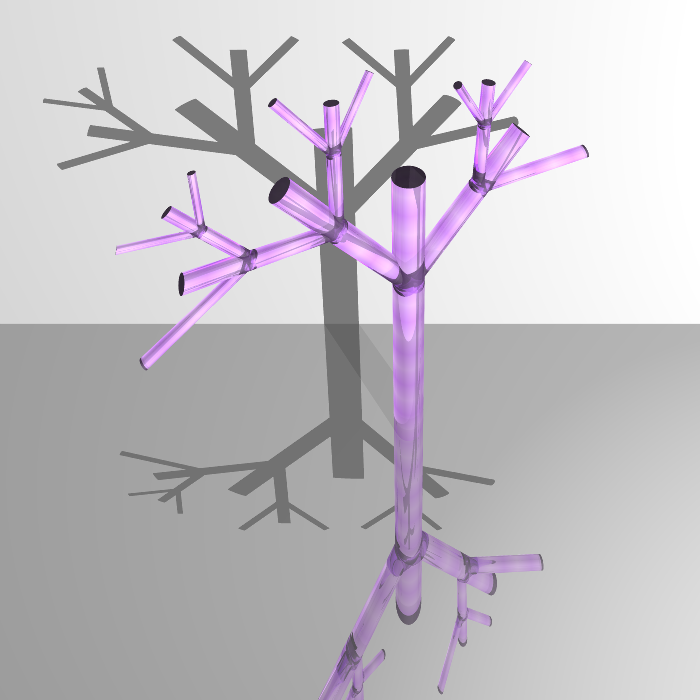
\includegraphics[scale=0.36]{tree.png}
\end{center}

\section{模型的局限性}
实验结果中的图片至少有2个地方不够真实.
\begin{compactitem}
\item 阴影的边缘是非常硬的, 但真实的图片中, 阴影边缘应该有一些缓慢过渡.
\item 圆柱状的透明物体, 如果它的材料是均匀的,
      那么它中间较厚的地方透明度应该比旁边较薄的小.
\end{compactitem}

这2个现象都是因为我们的模型设置导致的.
我们的模型是对真实光照模型的一个近似,
我们只考虑了物体的表面,
使得能够方便的用光线跟踪算法进行绘画.
如果想处理以上2个问题, 我们应该修改现在使用的模型.

\section{总结}
在这个实验中,
我实现了一个简单的光照模型.
并且结合上了第2章读书报告中, 关于消除锯齿的内容.
最终做出了一个较为理想的图片效果.

\end{document}
